\chapter{Numerische Methoden}
\section{Einleitung}
\section{GPGPU Computing mit CUDA}
\section{Finite Differenzen Verfahren}
\section{Validierung}
\newpage

\chapter{Immersed Boundary Methoden}

\begin{figure}[!bp]
  \centering
  \subfloat[kartesisches Gitter]{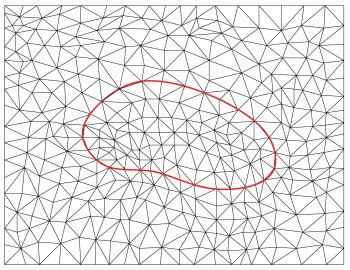
\includegraphics[width=0.4\textwidth]{gfx/immersed_boundary_methods/general_partition_triangle.jpg}\label{fig:f1}}
  \hfill
  \subfloat[unstrukturiertes Gitter]{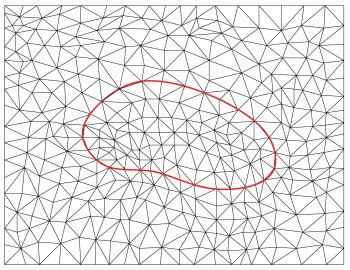
\includegraphics[width=0.4\textwidth]{gfx/immersed_boundary_methods/general_partition_triangle.jpg}\label{fig:f2}}
  \caption{Beispiele für numerische Gitter}
\end{figure}

\section{Einleitung}
Die bisher eingeführten Methoden eignen sich um auf einfachen Geometrien Simulationen durchzuführen.
Wenn die Ränder des Simulations-Gebietes nicht mehr mit dem numerischen Gitter übereinstimmen, lassen
sich die in Abschnitt () eingeführten Randbedingungen nicht mehr verwenden.
Das Problem lässt sich durch die Einführung eines an den Rand angepassten Gitter umgehen (s.Abb. \label{fig:f1}),
führt allerdings zu einem deutlich höheren Aufwand in den numerischen Berechnungen.
Die Berechnung des Gitters kann sehr aufwendig werden und es ist nicht eindeutig klar unter welchen
Performance-Einbussen sich das neue Gitter in der GPGPU-Implementierung verwenden lässt, da Bedingungen wie
z.B. Coalesced Readings  (s.Abbschnitt x) durch die unstrukturierten Daten deulich erschwert wären.
Eine Alternative die in dieser Arbeit verwendet wird sind  sog. Immersed Boundary Methoden.


- Beschreibung allgemein verschiedene immersed boundary methoden direkt /exp/ imp etc
    -erstmal peskin et al.
    -im prinzip 3 verschiedene ansätze continuous / direct /  ghost cell methoden
    - hier einfache methoden wegen gpu


- zunächst gehen wir nur auf den fall einer der geschwindigkeiten ein bllabla
Folgende Verfahren formel mit kraftterm
weiterer abschnitt temperatur / no-flux

\section{No-Slip-Boundaries}

\subsection{Volume Penalization}
-allgemeinsch beschreibung paper zitat, zitat dipl. lüllff.
-idee dämpungsterm in der dgl
-problem instabilität

\subsection{Direct Forcing}
-Paper quote
-vgl volume penalization warum keine instablilität
-formeln
-implementierung

\subsection{Direct Forcing mit Volume Fraction}
-paper quote formeln
-implementierung beispiel

\section{Direct Forcing mit Interpolation}
-paper quote formeln
-implementierung beispiel

\section{Methoden-Vergleich und numerische Validierung}
In diesem Abschnitt sollen die verschiedenen Methoden über numerische Testfälle validiert und miteinnander
verglichen werden.

\subsection{Validierung mit MASA}
-validierung mit masa für alle verfahren oben.. cube /evtl zylinder?
-vegl. und argumentation ränder ehh auf null.
-ein beispiel mit vol.pen.

\subsubsection{Planare Poiseuille Strömung}
Um die Dämfungseigenschaften der Volume-Penalization methode zu testen wurde zunächst ein planare Poiseuille-Strömung simuliert.
Der Aufbau ist in Abb. (x) dargestellt. Es handelt sich um eine laminare Strömung in x-Richtung die durch einen Druckgefälle $f=-\frac{\partial p}{\partial x}$ angetrieben wird.
Für die x- und y-Richtung werden periodische Randbedingungen angenommen, in z-Richtung gilt $\vec{v}(z=h_1) = \vec_{v}(z=h_2) = 0$.
Im stationären Fall lässt sich  die Bewegungsgleichung dann  auf eine Dimension reduzieren, es gilt:
\begin{align}
\frac{\partial v_x}{\partial t} &= - \frac{\partial p}{\partial x} + D \frac{\partial^2 v_x}{\partial z^2} = 0 \\
\Rightarrow v_x &= \frac{1}{2D}\frac{\partial p}{\partial x}z^2 + zc_1 + c_2\\
\end{align}
Mit $\vec{v}(h_1) = \vec_{v}(h_2) = 0$ und $A:=\frac{1}{2D}\frac{\partial p}{\partial x}$ ergibt sich:
\begin{align}
c_1 &= A\frac{h_1^2 -h_2^2}{h_2 - h_1} = -A(h_1+h_2)\\
c_2 &= A(h_1(h_1 + h_2) - h_1^2) = Ah_1h_2\\
\Rightarrow v_x &= A(z^2 - z(h_1 + h_2) + h_1h_2)
\end{align}
Da die Strömung in der Kanalmitte am stärksten ist gilt zudem:
\begin{align}
z_{max} &= \frac{h_1+h_2}{2}\Rightarrow v_{max} = A\left(h_1h_2 - \frac{(h_1 + h_2)^2}{4}\right)
\end{align}
Für die Strömung lässt sich die Reynoldszahl dann gemäß $Re \propto \frac{v_{max}}{D}$  bestimmen.








\subsubsection{Poiseuille Strömung im Zylinder}

\subsubsection{Zusammenfassung}


\subsection{No-Flux-Boundaries}

\subsubsection{'Variable Konduktivität'}










